\chapter{Bevezetés}\label{ch:introduction}

Ez a kézikönyv a \ReplicaGenOne{} és a \ReplicaNextLong{} digitális műszeregységeket ismerteti a Volkswagen Golf~II, Jetta~II és Scirocco~II modellekhez. Összefoglalja a hardverváltozatokat, bemutatja a funkciókat, és elmagyarázza a beszerelés, a konfigurálás, az üzemeltetés, a tárolás és a karbantartás lépéseit. Az útmutató járműtulajdonosoknak, autóvillamossági szakembereknek és olyan szervizeknek készült, amelyek utólag szerelik be a terméket.

A következő fejezetek ismertetik az azonosítási sémát, a csatlakozók kiosztását, az üzemi feltételeket, valamint a részletes beszerelési és konfigurációs eljárásokat. Mindkét Replica-generáció karbantartási és hibaelhárítási hivatkozásait is tartalmazza, hogy a műszeregység gyári dokumentáció nélkül is szakszerűen szervizelhető legyen.

\begin{figure}[htbp]
    \centering
    \begin{subfigure}{0.48\textwidth}
        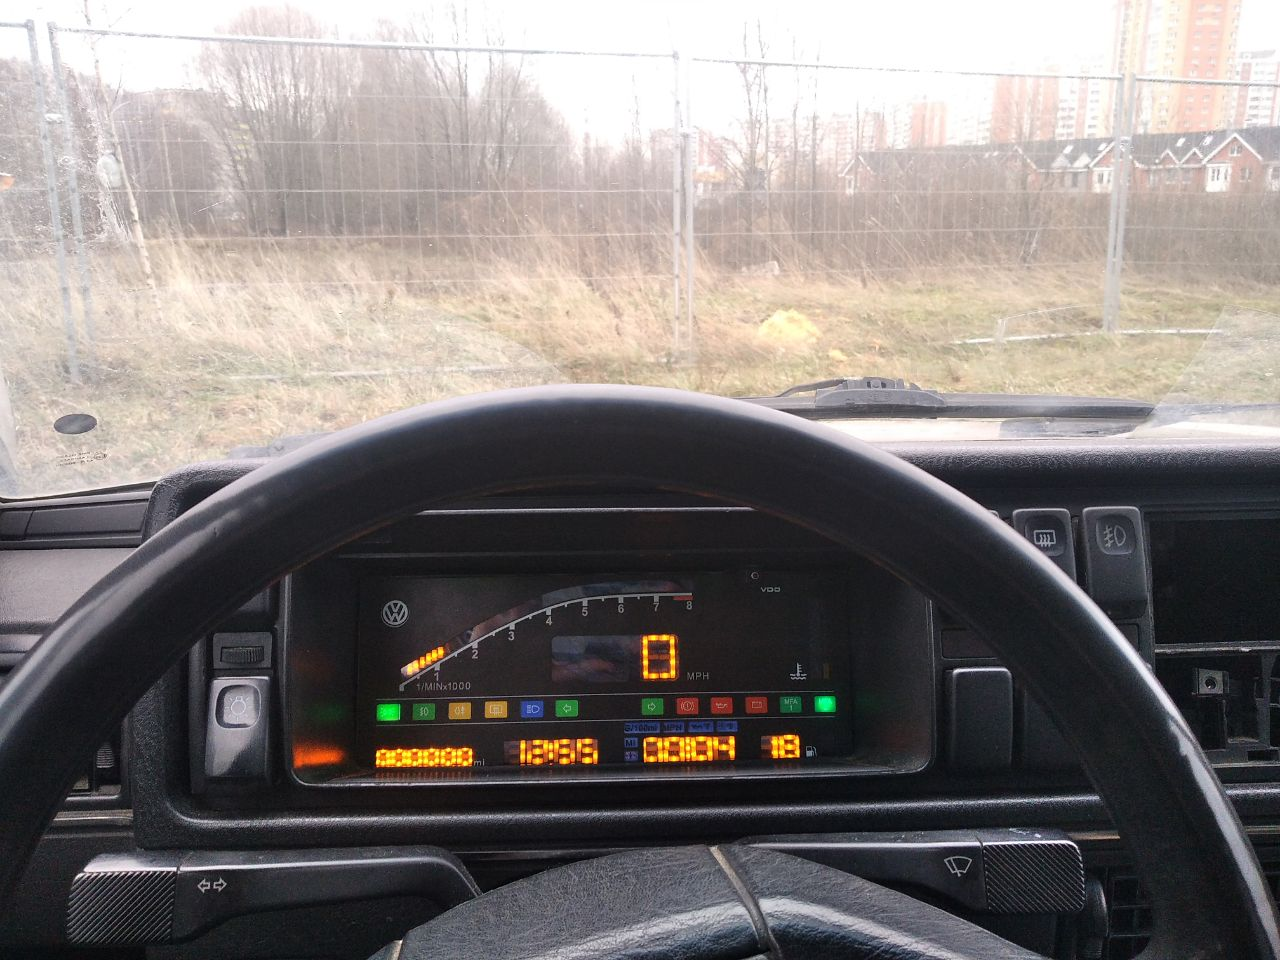
\includegraphics[width=\linewidth]{digifiz_manual/image004.jpg}
        \caption{Szállítási készlet a GART~8--MGF konfigurációhoz.}
    \end{subfigure}\hfill
    \begin{subfigure}{0.48\textwidth}
        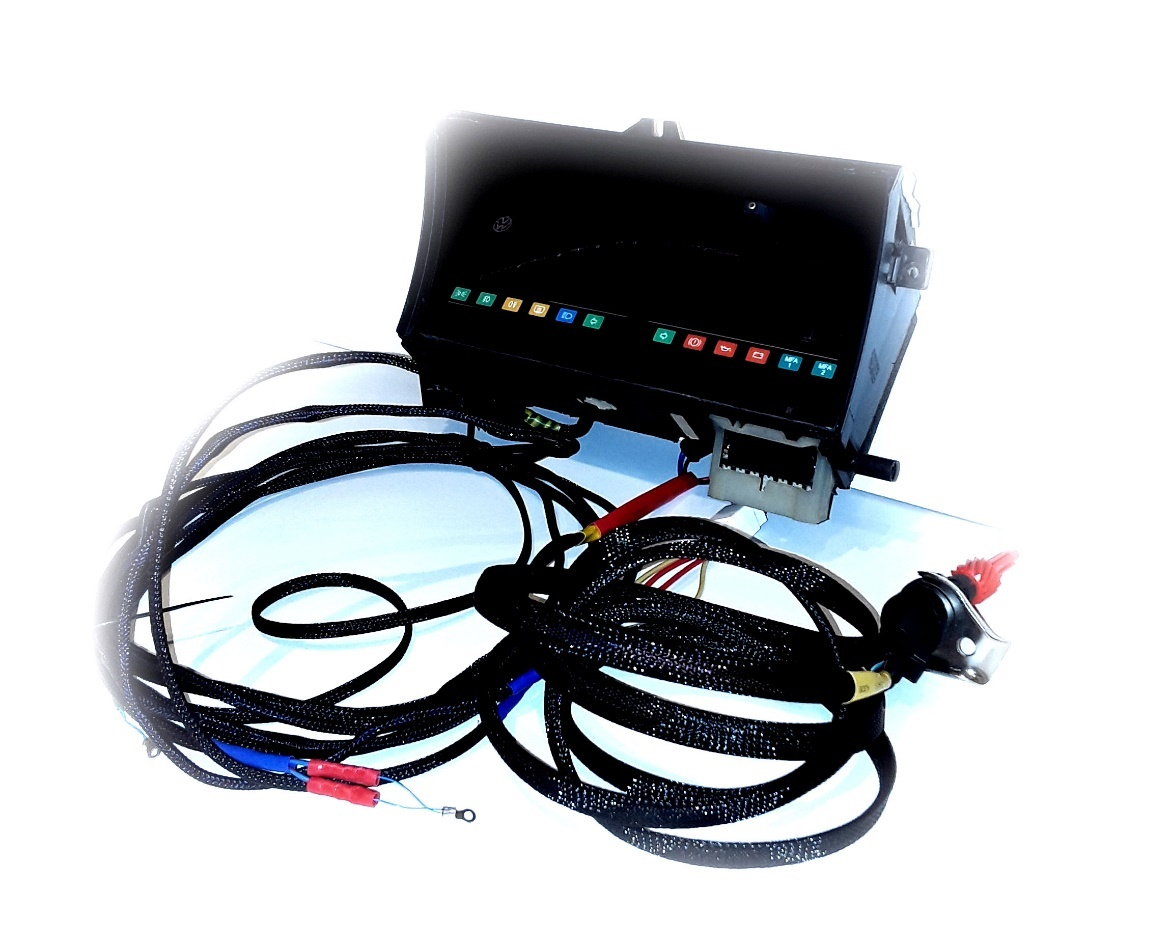
\includegraphics[width=\linewidth]{digifiz_manual/image005.jpg}
        \caption{Egy GART csomag tipikus tartalma.}
    \end{subfigure}
    \begin{subfigure}{0.48\textwidth}
        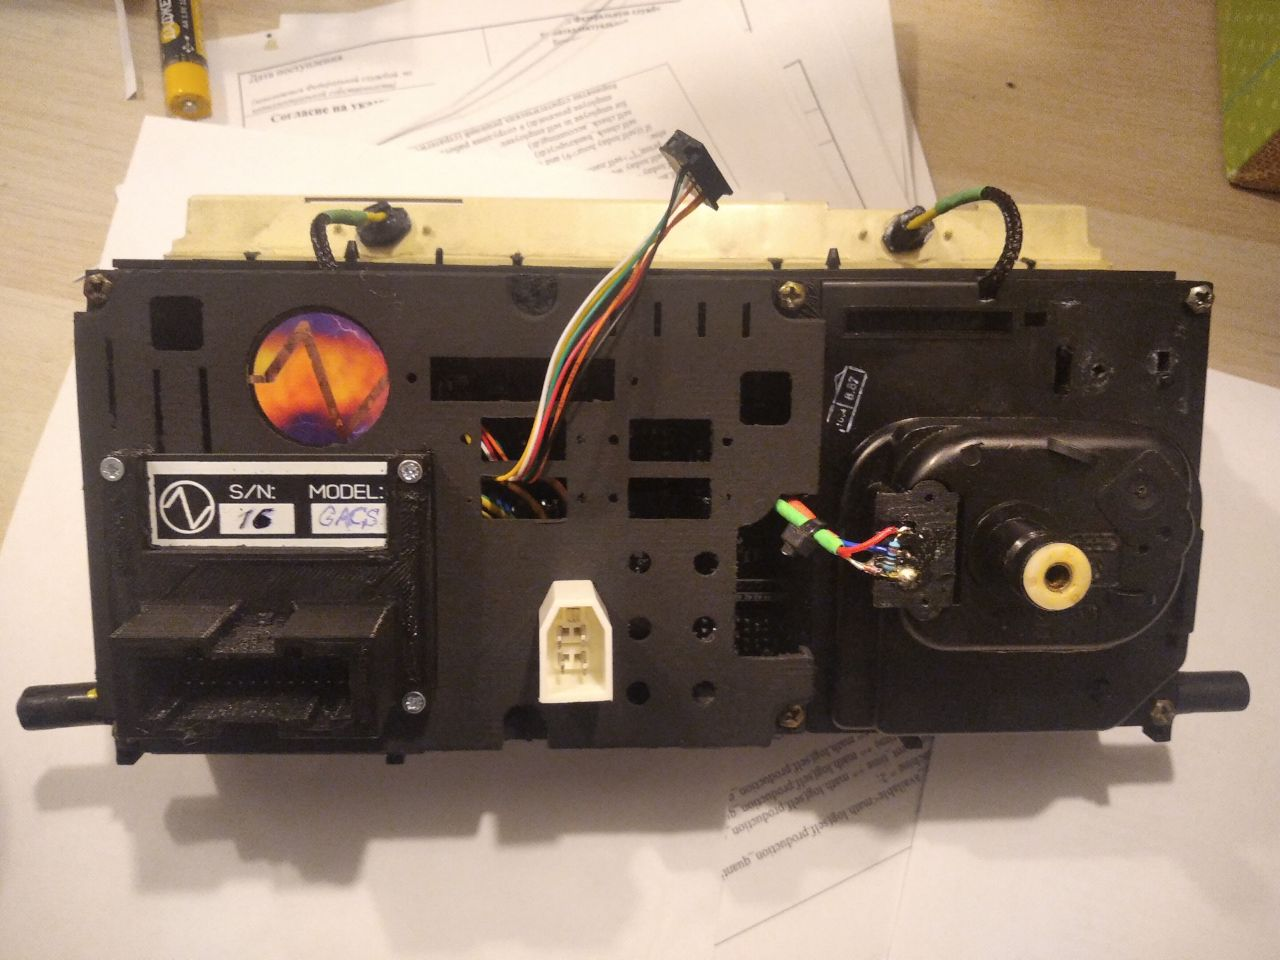
\includegraphics[width=\linewidth]{digifiz_manual/image006.jpg}
        \caption{A GACS összeállítás hátulnézete egyetlen csatlakozóval.}
    \end{subfigure}\hfill
    \begin{subfigure}{0.48\textwidth}
        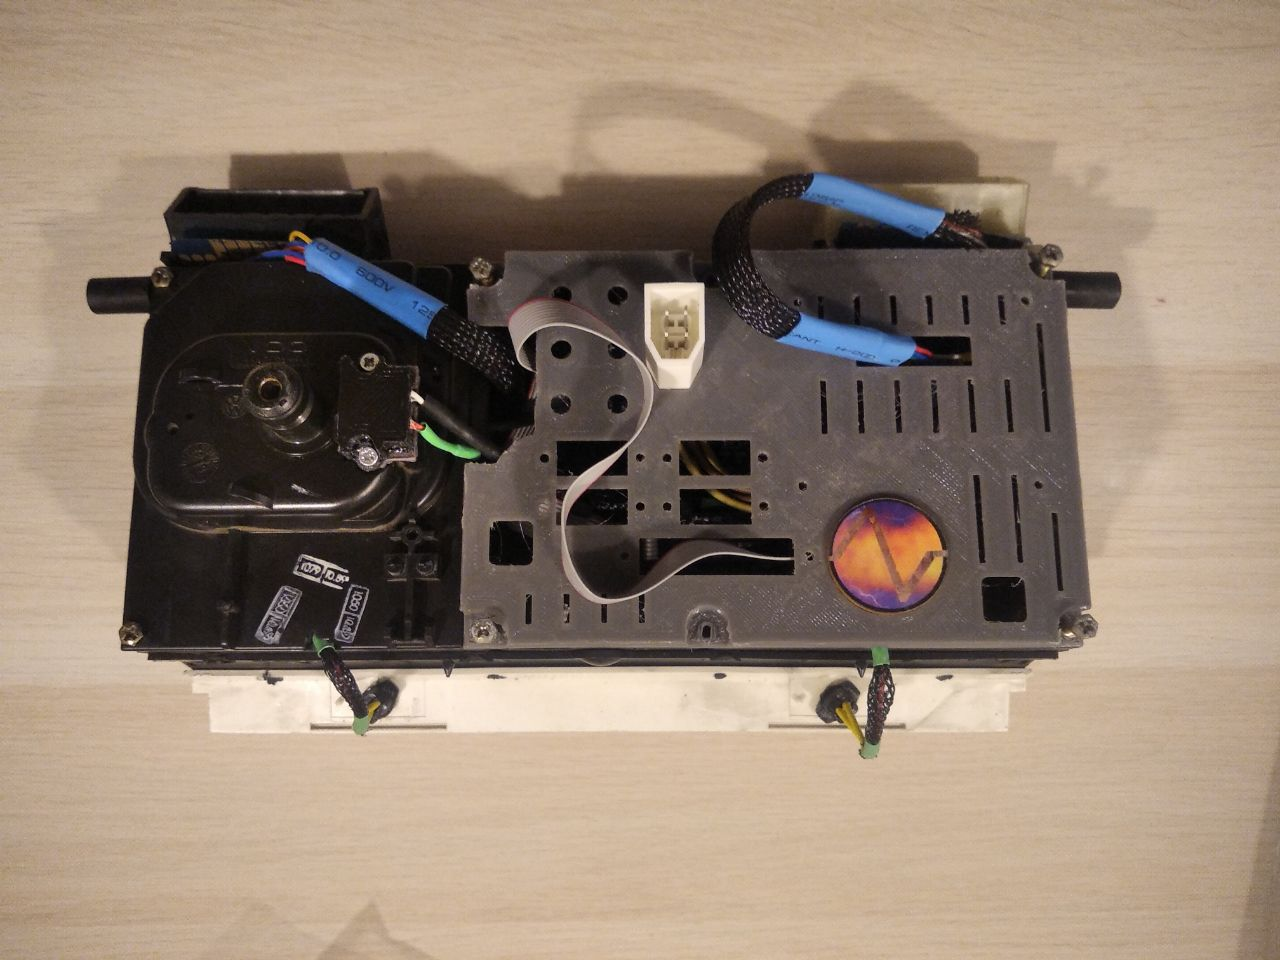
\includegraphics[width=\linewidth]{digifiz_manual/image007.jpg}
        \caption{A GACT összeállítás hátulnézete két csatlakozóval.}
    \end{subfigure}
    \caption{A kézikönyvhöz mellékelt \ReplicaGenOne{} és \ReplicaNextLong{} műszeregységek jellemző példái.}
\end{figure}

Minden változat az adott hajtáslánchoz, mértékegységhez és kábelkorbács-típushoz szükséges komponensekkel érkezik. A későbbi fejezetek részletezik a jelölések jelentését, és tartalmazzák a csatlakozótáblázatokat, hogy a műszeregység biztonságosan integrálható legyen.
